%%%%%%%%%%%%%%%%%%%%%%%%%%%%%%%%%%%%%%%%%%%%%%%%%%%%%%%%%%%%%%%%%%
%%%%%%%% ICML 2016 EXAMPLE LATEX SUBMISSION FILE %%%%%%%%%%%%%%%%%
%%%%%%%%%%%%%%%%%%%%%%%%%%%%%%%%%%%%%%%%%%%%%%%%%%%%%%%%%%%%%%%%%%

% Use the following line _only_ if you're still using LaTeX 2.09.
%\documentstyle[icml2016,epsf,natbib]{article}
% If you rely on Latex2e packages, like most moden people use this:
\documentclass{article}

% use Times
\usepackage{times}
% For figures
\usepackage{graphicx} % more modern
%\usepackage{epsfig} % less modern
\usepackage{subfigure}

% For citations
\usepackage{natbib}

% For algorithms
\usepackage{algorithm}
\usepackage{algorithmic}

% Maths
\usepackage{amsmath}
\usepackage{amssymb}

% As of 2011, we use the hyperref package to produce hyperlinks in the
% resulting PDF.  If this breaks your system, please commend out the
% following usepackage line and replace \usepackage{icml2016} with
% \usepackage[nohyperref]{icml2016} above.
\usepackage{hyperref}

% Packages hyperref and algorithmic misbehave sometimes.  We can fix
% this with the following command.
\newcommand{\theHalgorithm}{\arabic{algorithm}}

% Employ the following version of the ``usepackage'' statement for
% submitting the draft version of the paper for review.  This will set
% the note in the first column to ``Under review.  Do not distribute.''
% \usepackage{icml2016}

% Employ this version of the ``usepackage'' statement after the paper has
% been accepted, when creating the final version.  This will set the
% note in the first column to ``Proceedings of the...''
\usepackage[accepted]{icml2016}


% The \icmltitle you define below is probably too long as a header.
% Therefore, a short form for the running title is supplied here:
\icmltitlerunning{Deep Manifold Learning on Music Audio for Navigating Large Sound Libraries}

\begin{document}

\twocolumn[
\icmltitle{Deep Manifold Learning on Music Audio \\
           for Navigating Large Sound Libraries}

% It is OKAY to include author information, even for blind
% submissions: the style file will automatically remove it for you
% unless you've provided the [accepted] option to the icml2016
% package.
\icmlauthor{Eric J. Humphrey}{ejhumphrey@spotify.com}
\icmladdress{Spotify USA,
            620 Avenue of the Americas, New York City, NY 10011 USA}
% \icmlauthor{Your CoAuthor's Name}{email@coauthordomain.edu}
% \icmladdress{Their Fantastic Institute,
%             27182 Exp St., Toronto, ON M6H 2T1 CANADA}

% You may provide any keywords that you
% find helpful for describing your paper; these are used to populate
% the "keywords" metadata in the PDF but will not be shown in the document
\icmlkeywords{boring formatting information, machine learning, ICML}

\vskip 0.3in
]

\begin{abstract}

In this talk, we explore the application of manifold learning with solo instrument samples to yield low-dimensional representations of sound for visualization and browsing.
Our approach uses deep neural networks to jointly learn features and an embedding space, trained to optimally preserve neighborhood relationships.
We then turn our attention to evaluating the usefulness of the resulting embeddings, both through quantitative benchmarking and exploring notable multimedia examples.


\end{abstract}

\section{Introduction}
\label{submission}

% A query for ``voice'' returns over 19k results on FreeSound, a collaborative database of audio clips.

Navigating large sound libraries has long been a pain point for musicians, artists, and producers.
Search queries are predominantly forced to take the form of text, which is problematic for at least two reasons.
Metaphors and descriptive tags, when provided, struggle to capture nuanced characteristics in sufficient detail, and this language often varies from one individual to the next.
Alternatively, standard approaches to sound visualization -- waveform envelopes or spectrograms -- are hardly intuitive for the general population.
% Furthermore, such descriptions are not always associated with every sound in a collection, and typically only at the granularity of the entire recording.
% As a result, the task of navigating a sound library is often reduced to that of an exhaustive, brute force search.
As a result, the development of computational systems for acoustic similarity, an elusive concept in its own right, remains an open research topic.

% The link between ^ and v isn't stellar.
Acoustic similarity is a natural use case for manifold learning, which attempts to preserve relationships in a low dimensional space, often for visualization.
Common embedding methods, such as Multidimensional Scaling (MDS) \cite{borg2005mds}, Locally Linear Embedding (LLE) \cite{roweis2000nonlinear}, or Isomap \cite{tenenbaum2000global}, respect pairwise distances between observations, but exhibit two practical drawbacks:
these methods do not yield general functions that can be applied to new data, and obtaining accurate pairwise distances for large datasets is not scalable.
Ranking methods, like WSABIE \cite{weston2011wsabie}, relax this constraint in favor of maintaining relative order between observations, but these nuanced relationships can still be hard to obtain at scale.
Neighborhood methods, such as neighborhood components analysis (NCA) \cite{goldberger2004neighbourhood, salakhutdinov2007learning}, DrLIM \cite{hadsell2006dimensionality}, or \texttt{word2vec}
% ~\footnote{Note that \texttt{word2vec} is strictly an embedding model, and not a functional mapping.}
\cite{mikolov2013distributed}, simplifiy the problem even further by exploiting unordered set relationships.
Rather than placing the burden of continuity on the data, neighborhood methods task the model with smoothly interpolating discrete sets in the embedding space.
 % easier to obtain, especially from large datasets, or be defined by coarse \emph{a priori} knowledge, \emph{e.g.} descriptive tags.
Prior work has demonstrated the potential for such methods to yield intutitive representations, where algebraic operations on vectors encode physical orientation \cite{hadsell2006dimensionality} or analogy \cite{mikolov2013efficient}.

Synthesizing these two topics, neighborhood-based ``deep'' manifold learning methods have shown promise in producing intuitive acoustic representations from sound samples \cite{humphrey2011nlse}, and we extend that work here.
% Different kinds of neighborhoods are easy to draw from data, and we are curious to examine the different mappings they produce.
Deep neural networks provide a general approach to mapping high-dimensional data into useful embeddings, which we influence by considering different relationships between inputs.
% Feature learning is particularly important for acoustic similarity, as the perceptual quality of ``timbre'' remains an ill-defined concept.
Semantic organization of the learned embeddings can be demonstrated through various means, such as nearest-neighbor classification and visual exploration.


\section{Method}

We approach acoustic similarity by optimizing the parameters of a deep neural network to maximally preserve $K$ contrasting set relationships, \emph{i.e.} neighborhoods, between samples in a low-dimensional Euclidean space.
Given a collection of observations, $\mathcal{D}$, the $k^{th}$ contrastive parition consists of a positive, $\Gamma_k$, and a negative, $\bar{\Gamma_k}$, subset, satisfying three conditions:
one, contrastive partitions are internally disjoint, $\Gamma_k \cap \bar{\Gamma_k} = \varnothing$;
two, contrastive partitions may comprise a subset of the entire collection, $|\Gamma_k \cup \bar{\Gamma_k}| \le |\mathcal{D}|$;
and three, contrastive partitions are drawn independently of each other, such that any two partitions, $i$ and $j$, may share observations, $|\Gamma_i \cap \Gamma_j| \ge 0$.
Thus, the network can be understood as interpolating the various discrete partitions, with the training objective finding a smooth compromise between them.


\subsection{Model}

The model used here follows prior work \cite{humphrey2015dl4mir}.
Audio is first transformed to a constant-Q representation, parameterized as follows:
signals are downsampled to 16kHz;
bins are spaced at 24 per octave, or quarter-tone resolution, and span eight octaves, from 27.5Hz to 7040Hz;
analysis is performed at a framerate of 20Hz.
Logarithmic compression is applied to the frequency coefficients, i.e. $log(C*X + 1.0)$, with $C=50$.
Multi-frame windows are transformed by a five-layer convolutional neural network (CNN) into a 3-dimensional vector.
The network consists of three 3D-convolutional layers and two fully connected layers, with max-pooling by 2 in time for first two layers.
The first four layers use hyperbolic tangent activation functions, while the last layer is linear to avoid saturation.


\subsection{Learning a Mapping into Euclidean Space}

% Loss architecture
A contrastive loss function is used to optimize the model's parameters,
% in line with related work \cite{humphrey2011nlse, humphrey2015dl4mir}.
with copies of the model arranged in a ternary configuration, defined as follows:

% loss_sim = hwr(cost_sim - margin_sim)^2
% loss_diff = hwr(margin_diff - cost_diff)^2
% total = ave(loss_sim + loss_diff)
\vspace{-0.15in}
\begin{align*}
Z_i = \mathcal{F}(X_i | \Theta),~Z_p = \mathcal{F}(X_p | \Theta),~Z_n = \mathcal{F}(X_n | \Theta)\\
D_p = || Z_i - Z_p ||_2,~D_n = || Z_i - Z_n ||_2\\
\mathcal{L} = \max(0, D_p - m_{p})^2 + \max(0, m_{n} - D_n)^2 \\
\end{align*}
\vspace{-0.3in}


Here, three observations, $X_i$, $X_p$, $X_n$, are transformed by the model, $\mathcal{F}$, given the same parameters, $\Theta$.
These observations are chosen such that $X_i, X_p \in \Gamma_k$ and $X_n \in \bar{\Gamma_k}$.
Euclidean distance is computed between embedding pairs, and two margins, $m_p$ and $m_n$, define thresholds on their respective loss terms.
Parameters are learned via minibatch stochastic gradient descent with a batch size of 32, and training proceeded for 50k iterations.

\subsection{Data}

% The data source used herein is drawn from the Vienna Symphonic Library (VSL), a massive collection of studio-grade orchestral instrument samples recorded over a variety of performance techniques\footnote{\url{https://vsl.co.at/en}}.
We use a previously compiled collection of solo instrument samples, comprised of 5k instances drawn from 24 instrument classes \cite{humphrey2015dl4mir}.
The set is partitioned into 72k, 18k, and 30k for training, validation, and testing, respectively.
The crux of this exploration lies in \emph{how} neighborhoods are defined and sampled for training, and thus various relationships are considered to encourage different kinds of embeddings, including instrument class, absolute pitch, instrument class and absolute pitch, and instrument class and absolute pitch $\pm~2$ semitones.
% \item Instrument class and pitch chroma


\section{Evaluation}

We consider a few approaches to measuring the quality of the learned acoustic embeddings, provided in greater detail elsewhere.\footnote{\url{https://github.com/ejhumphrey/icml16-dml}}
% Neighbors
Quantitatively, $k$-nearest neighbor classification measures the extent to which neighborhoods are preserved, and brute-force distance is used to sort data in a ranked retrieval setting.
% Overall we find the learned embeddings are well-organized and consistently demonstrate robust performance in query-by-example tasks.
% Consistent with previous results \cite{humphrey2011nlse, humphrey2015dl4mir}, the sharpness of class boundaries is inversely to the discrete number of neighborhoods, and is likely due in part to the limits of three-space.
% Analogy
These representations additionally lend themselves well to visualization and sonification.
Scatterplots reveal some surprising behavior, as in Figure \ref{fig:asdr}, where an attack-decay-sustain-release (ADSR) envelope is made apparent by following the evolution of sounds through space.
% Acoustic ``analogy'' serves as an interesting test of semantic organization, where the resultant vector between two points is applied to a third.
Finally, sound trajectories are sonified via concatenative synthesis, providing audible insight into the learned embeddings.



\begin{figure}[!t]
\vskip -0.35in
\begin{center}
\centerline{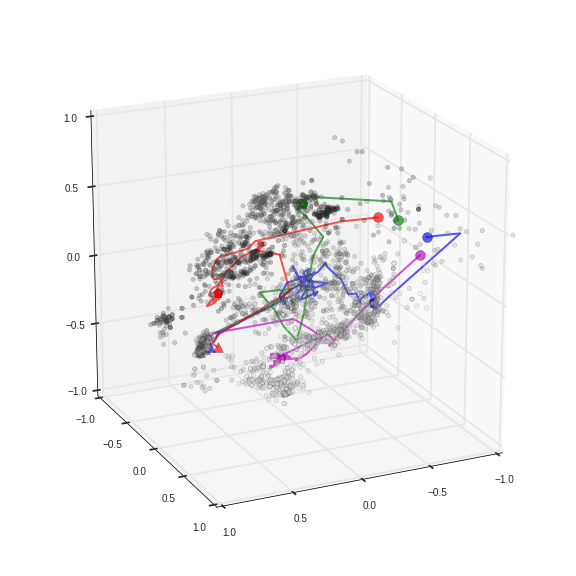
\includegraphics[width=3.1in]{inst-pitch-d2_adsr.pdf}}
\vskip -0.2in
\caption{An embedding where random samples (grayscale) show pitch height from low (black) to high (white) and four sounds are shown from start (cirlces) to end (triangles): trumpet (blue), trombone (green), tenor saxophone (red) and clarinet (magenta).}
\label{fig:asdr}
\end{center}
\vskip -0.25in
\end{figure}



\section{Summary}

% Here's what we did
A range of acoustic embeddings are learned using a convolutional neural network optimized to preserve different neighborhood relationships between instrument sounds in 3-space.
% Here's what we found
The learned embeddings demonstrate a useful degree of semantic organization, indicated by performance on retrieval tasks and notable multimedia examples.
% Here's where we're going
In doing so, we hope to further motivate the role of sound visualization in music discovery, how deep networks can help address this challenge, and the potential this area holds for future exploration.
% Novel interactions with sound and music.


\bibliography{example_paper}
\bibliographystyle{icml2016}

\end{document}
